\documentclass[11pt,a4paper,DIV9,BCOR1.5mm,twoside]{scrartcl}
\usepackage{import}
\subimport*{}{packages/Bericht_Hoch.tex}
\subimport*{}{packages/colors.tex}
\begin{document}


\begin{knitrout}
\definecolor{shadecolor}{rgb}{0.969, 0.969, 0.969}\color{fgcolor}\begin{kframe}
\begin{alltt}
\hlkwd{setwd}\hlstd{(}\hlstr{"C:/lucmiaz/algorithms-analysis-report"}\hlstd{)}
\hlkwd{library}\hlstd{(jsonlite)}
\hlkwd{library}\hlstd{(ggplot2)}
\hlkwd{library}\hlstd{(dplyr)}
\hlkwd{library}\hlstd{(RColorBrewer)}
\hlkwd{library}\hlstd{(extrafont)}
\hlkwd{require}\hlstd{(tikzDevice)}
\hlkwd{loadfonts}\hlstd{()}
\hlstd{json_file}\hlkwb{=}\hlstr{"Datamaous.json"}
\hlstd{csv_file}\hlkwb{=}\hlstr{"Datamaous.csv"}
\hlstd{tf}\hlkwb{<-}\hlkwd{read.csv}\hlstd{(csv_file)}
\hlkwd{remove}\hlstd{(json_file)}
\hlcom{#clusters<-kmeans(tf$spec,1000)}
\hlcom{#tf[,'cluster']<-clusters$cluster}
\hlcom{#to do add clusters$cluster column to tf and then merge by groups...}
\hlcom{#tf<-cbind()}
\end{alltt}
\end{kframe}
\end{knitrout}

\begin{figure}
\begin{knitrout}
\definecolor{shadecolor}{rgb}{0.969, 0.969, 0.969}\color{fgcolor}\begin{kframe}
\begin{alltt}
\hlcom{#tikz('normal.tex', standAlone = TRUE, width=5, height=5)}
\hlstd{theme_bw}\hlkwb{<-}\hlkwd{theme_update}\hlstd{(}\hlkwc{text}\hlstd{=}\hlkwd{element_text}\hlstd{(}\hlkwc{size}\hlstd{=}\hlnum{14}\hlstd{,} \hlkwc{family}\hlstd{=}\hlstr{"Helvetica Neue"}\hlstd{),} \hlkwc{axis.text}\hlstd{=}\hlkwd{element_text}\hlstd{(}\hlkwc{family}\hlstd{=}\hlstr{"Helvetica Neue"}\hlstd{),}\hlkwc{legend.background}\hlstd{=}\hlkwd{element_rect}\hlstd{(}\hlkwc{fill}\hlstd{=}\hlstr{"#f5f5f5"}\hlstd{))}
\hlkwd{theme_set}\hlstd{(}\hlkwd{theme_bw}\hlstd{())}
\hlcom{#barplot<-ggplot(data=subset(tf, cluster %in% arrange(cluster, desc(cluster))[1:4,]), aes(spec, fill=as.factor(cluster)))+}
\hlstd{barplot}\hlkwb{<-}\hlkwd{ggplot}\hlstd{(}\hlkwc{data}\hlstd{=}\hlkwd{filter}\hlstd{(tf, tf}\hlopt{$}\hlstd{author}\hlopt{!=}\hlstr{'esr'} \hlopt{&} \hlstd{tf}\hlopt{$}\hlstd{quality}\hlopt{!=}\hlnum{1}\hlstd{),} \hlkwd{aes}\hlstd{(disct, spec,} \hlkwc{fill}\hlstd{=}\hlkwd{as.factor}\hlstd{(disct)))}\hlopt{+}\hlkwd{geom_violin}\hlstd{(}\hlkwc{stat} \hlstd{=} \hlstr{"ydensity"}\hlstd{,} \hlkwc{position} \hlstd{=} \hlstr{"dodge"}\hlstd{)}\hlopt{+}
\hlcom{#geom_histogram(binwidth=0.2,alpha = 0.4, position = 'identity')+}
  \hlkwd{xlab}\hlstd{(}\hlstr{"Element was selected as flanging"}\hlstd{)} \hlopt{+} \hlkwd{ylab}\hlstd{(}\hlstr{"BPR"}\hlstd{)}\hlopt{+}
  \hlkwd{coord_flip}\hlstd{()}\hlopt{+}\hlcom{#rotates the graphic}
  \hlkwd{facet_wrap}\hlstd{(algprop}\hlopt{~}\hlstd{author,} \hlkwc{scales}\hlstd{=}\hlstr{'free'}\hlstd{)}\hlopt{+}\hlcom{#plots by author}
  \hlkwd{scale_fill_brewer}\hlstd{(}\hlkwc{type}\hlstd{=}\hlstr{'div'}\hlstd{)}\hlcom{#colorscale}
\hlkwd{ggsave}\hlstd{(}\hlstr{"figures/BPRAuthorAlgprops.pdf"}\hlstd{,} \hlkwc{plot}\hlstd{=barplot,}  \hlkwc{width}\hlstd{=}\hlnum{20}\hlstd{,} \hlkwc{height}\hlstd{=}\hlnum{20}\hlstd{)}
\end{alltt}


{\ttfamily\noindent\bfseries\color{errorcolor}{\#\# Error in facet\_render.wrap(plot\$facet, panel, plot\$coordinates, plot\_theme(plot), : ggplot2 does not currently support free scales with a non-cartesian coord or coord\_flip.}}\begin{alltt}
\hlstd{barplot}
\end{alltt}


{\ttfamily\noindent\bfseries\color{errorcolor}{\#\# Error in facet\_render.wrap(plot\$facet, panel, plot\$coordinates, plot\_theme(plot), : ggplot2 does not currently support free scales with a non-cartesian coord or coord\_flip.}}\begin{alltt}
\hlcom{#dev.off()}
\end{alltt}
\end{kframe}
\end{knitrout}
\end{figure}






\Sconcordance{concordance:Zischendetetkt2.tex:Zischendetetkt2.Rnw:%
1 2 1 1 0 1 1 1 2 1 0 9 1 1 6 5 0 1 1 3 0 1 2 1 4 1 2 1 1 1 3 1 2 3 1}

\begin{Schunk}
\begin{Sinput}
> library(jsonlite)
> library(ggplot2)
> library(dplyr)
> library(RColorBrewer)
> json_file<-'C:/LucMiaz/KG_dev_branch/KG/Measurements_example/MBBMZugExample/results/test_ZischenDetetkt2_2.0s_3000Hz_0dB_20-10-2015_14-59-39.json'
> dataraw<-fromJSON(json_file)
> tf<-dataraw$R
> tf <- filter(tf, !is.nan(BPR))
> tprfpr <- data.frame(TPR=double(), FPR=double(),threshold=double())
> authors=paste(unique(tf$author), sep=", ")
> for(i in seq(0.1,1,0.01)){
+   result<- tf$BPR<i
+   tf<-tf %>% mutate_(leqBPR=paste(as.numeric(result)))
+   len<-length(tf$leqBPR[!is.na(tf$leqBPR)])
+   tprfpr <- rbind(tprfpr,data.frame(TPR=sum(tf$leqBPR[tf$disc==1 & !is.na(tf$leqBPR)])/len, FPR=sum(tf$leqBPR[tf$disc==0 &!is.na(tf$leqBPR)])/len, threshold=i))
+ }
> tf$leqBPR<- NULL
\end{Sinput}
\end{Schunk}
\begin{figure}
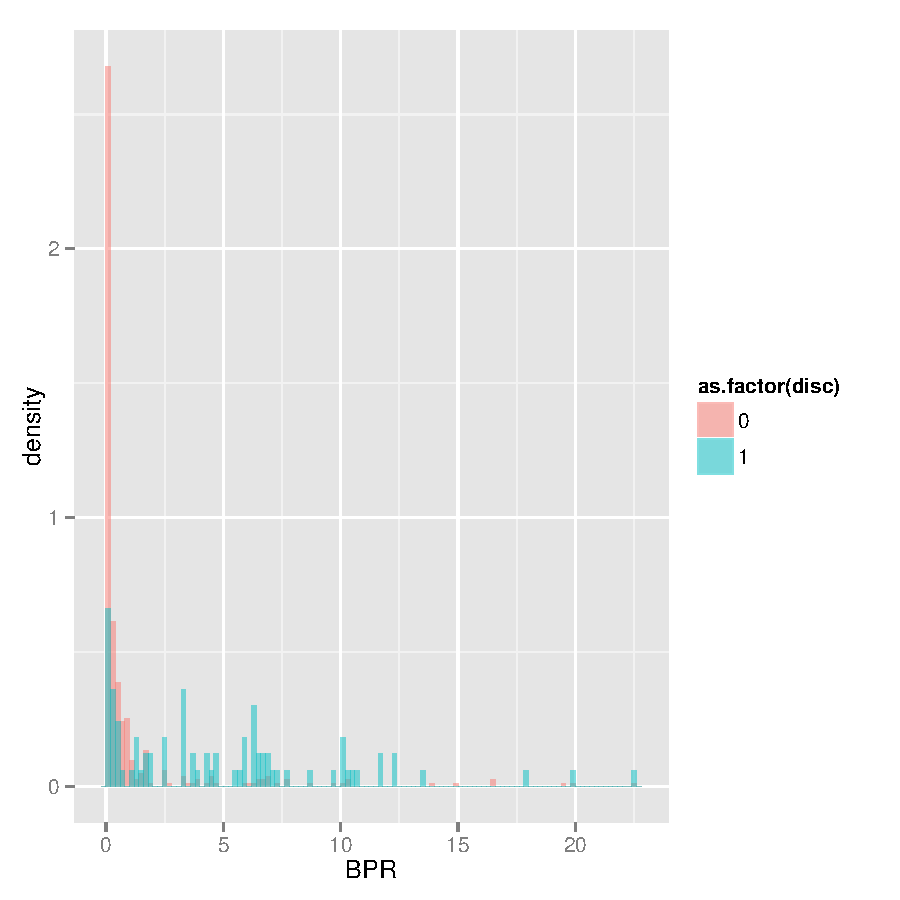
\includegraphics{Zischendetetkt2-002}
\end{figure}
\begin{figure}
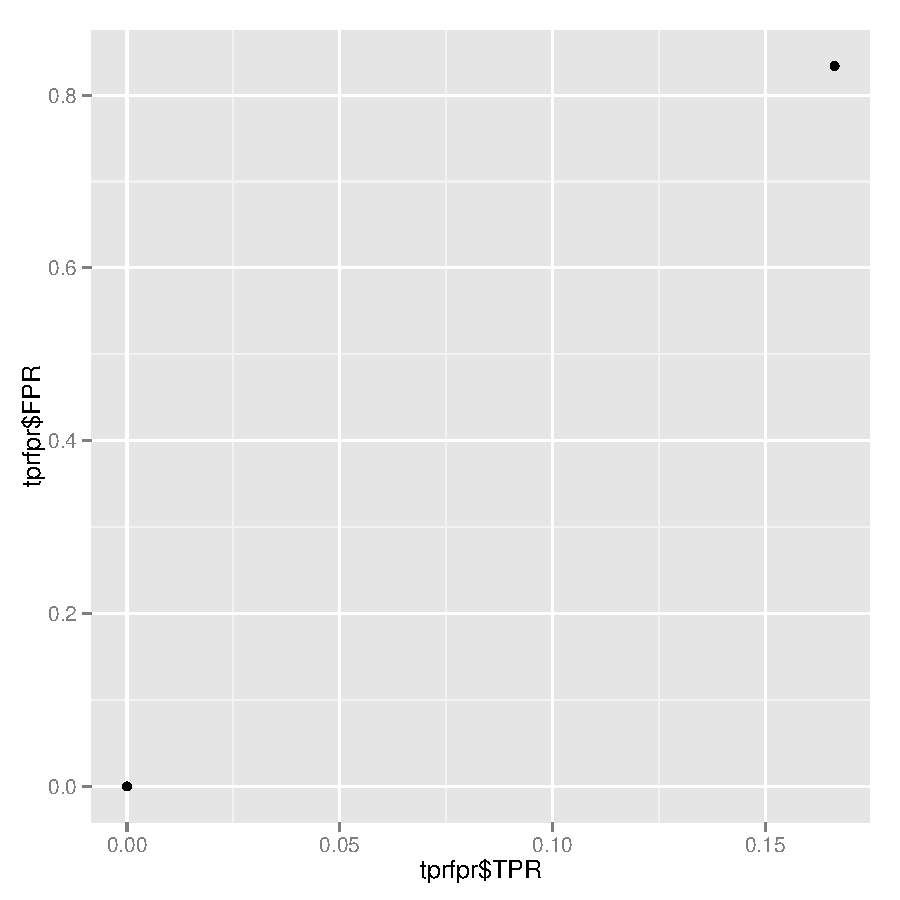
\includegraphics{Zischendetetkt2-003}
\end{figure}